%%%%%%%%%%%%%%%%%%%%%%%%%%%%%%%%%%%%%%%%%
% Structured General Purpose Assignment
% LaTeX Template
%
% This template has been downloaded from:
% http://www.latextemplates.com
%
% Original author:
% Ted Pavlic (http://www.tedpavlic.com)
%
% Note:
% The \lipsum[#] commands throughout this template generate dummy text
% to fill the template out. These commands should all be removed when
% writing assignment content.
%
%%%%%%%%%%%%%%%%%%%%%%%%%%%%%%%%%%%%%%%%%

%----------------------------------------------------------------------------------------
%	PACKAGES AND OTHER DOCUMENT CONFIGURATIONS
%----------------------------------------------------------------------------------------

\documentclass[12pt]{article}

\usepackage{fancyhdr,lastpage,extramarks,graphicx,booktabs,marvosym,xcolor,hyperref,graphicx}
\usepackage[most]{tcolorbox}
\usepackage{caption}
\usepackage{subcaption}
\usepackage{framed}

\usepackage{sectsty}

\allsectionsfont{\centering}
% Margins
\topmargin=-0.45in
\evensidemargin=0in
\oddsidemargin=0in
\textwidth=6.5in
\textheight=9.0in
\headsep=0.25in

\linespread{1.1} % Line spacing

% Set up the header and footer
\pagestyle{fancy}
\lhead{\hmwkAuthorName} % Top left header
\chead{\hmwkClass\ (\hmwkClassInstructor\ \hmwkClassTime): \hmwkTitle} % Top center header
\rhead{\firstxmark} % Top right header
\lfoot{\lastxmark} % Bottom left footer
\cfoot{} % Bottom center footer
\rfoot{Page\ \thepage\ of \pageref{LastPage}} % Bottom right footer
\renewcommand\headrulewidth{0.4pt} % Size of the header rule
\renewcommand\footrulewidth{0.4pt} % Size of the footer rule

%----------------------------------------------------------------------------------------
%	DOCUMENT STRUCTURE COMMANDS
%	Skip this unless you know what you're doing
%----------------------------------------------------------------------------------------

% Header and footer for when a page split occurs within a problem environment
\newcommand{\enterProblemHeader}[1]{%
    \nobreak\extramarks{#1}{#1 continued on next page\ldots}\nobreak%
    \nobreak\extramarks{#1 (continued)}{#1 continued on next page\ldots}\nobreak%
}

% Header and footer for when a page split occurs between problem environments
\newcommand{\exitProblemHeader}[1]{%
    \nobreak\extramarks{#1 (continued)}{#1 continued on next page\ldots}\nobreak%
    \nobreak\extramarks{#1}{}\nobreak%
}

\setcounter{secnumdepth}{0} % Removes default section numbers
\newcounter{homeworkProblemCounter} % Creates a counter to keep track of the number of problems

\newcommand{\homeworkProblemName}{}
\newenvironment{homeworkProblem}[1][Problem \arabic{homeworkProblemCounter}]{ % Makes a new environment called homeworkProblem which takes 1 argument (custom name) but the default is "Problem #"
    \stepcounter{homeworkProblemCounter} % Increase counter for number of problems
    \renewcommand{\homeworkProblemName}{#1} % Assign \homeworkProblemName the name of the problem
    \section{\homeworkProblemName} % Make a section in the document with the custom problem count
    \enterProblemHeader{\homeworkProblemName} % Header and footer within the environment
    }{%
    \exitProblemHeader{\homeworkProblemName} % Header and footer after the environment
}

\newcommand{\problemAnswer}[1]{% Defines the problem answer command with the content as the only argument
    \begin{tcolorbox}[colback=black!5!white,colframe=black!75!black]
        \centering
    \begin{minipage}{0.98\columnwidth}#1\end{minipage}
    \end{tcolorbox} % Makes the box around the problem answer and puts the content inside
}

\newcommand{\homeworkSectionName}{}
\newenvironment{homeworkSection}[1]{ % New environment for sections within homework problems, takes 1 argument - the name of the section
    \renewcommand{\homeworkSectionName}{#1} % Assign \homeworkSectionName to the name of the section from the environment argument
    \subsection{\homeworkSectionName} % Make a subsection with the custom name of the subsection
    \enterProblemHeader{\homeworkProblemName\ [\homeworkSectionName]} % Header and footer within the environment
    }{%
    \enterProblemHeader{\homeworkProblemName} % Header and footer after the environment
}

%----------------------------------------------------------------------------------------
%	NAME AND CLASS SECTION
%----------------------------------------------------------------------------------------

\newcommand{\hmwkTitle}{Test \#2} % Assignment title
\newcommand{\hmwkDueDate}{Wednesday, May\ 10\textsuperscript{th},\ 2017} % Due date
\newcommand{\hmwkClass}{PHILOS\ 3235} % Course/class
\newcommand{\hmwkClassTime}{15:00} % Class/lecture time
\newcommand{\hmwkClassInstructor}{Dittmer} % Teacher/lecturer
\newcommand{\hmwkAuthorName}{Illya Starikov} % Your name

%----------------------------------------------------------------------------------------
%	TITLE PAGE
%----------------------------------------------------------------------------------------

\title{%
    \vspace{2in}
    \textmd{\textbf{\hmwkClass:\ \hmwkTitle}}\\
    \normalsize\vspace{0.1in}\small{Due\ on\ \hmwkDueDate}\\
    \vspace{0.1in}\large{\textit{\hmwkClassInstructor\ \hmwkClassTime}}
    \vspace{3in}
}

\author{\textbf{\hmwkAuthorName}}
\date{Monday, April 3\textsuperscript{rd}, 2017} % Insert date here if you want it to appear below your name

%----------------------------------------------------------------------------------------

\begin{document}
\maketitle\newpage

\begin{homeworkProblem}[Problem \Roman{homeworkProblemCounter}] % Roman numerals
    \problemAnswer{% Answer
        Utilitarianism states that actions are right just in case they produce the most overall (available) goodness.  Discuss some ways in which according to Kantian ethics, utilitarianism is false.
    }
    Utilitarianism and Kantian ethics seem to have have a large overlap. After all, utilitarianism is the doctrine that actions are right if they benefit the majority and Kantian Ethics reflect much of this thinking. However, when analyzing the two frameworks of ethics, there are areas where they differ. The biggest area of difference is in the first Categorical Imperative.

    The first Categorical Imperative states that

    \begin{quote}
        Act only according to that maxim by which you can at the same time will that it should become a universal law.
    \end{quote}

    This may seem like a perfect utilitarian definition; until one realizes that ``universal'' is not the same as ``maximum benefit''. To show how this juxtaposition is true, let us take two examples.

    One of the most widely known examples of a wrong in Kantian Ethics is suicide. If everyone committed suicide (making it universal), the human-centric ethics would fall apart. However, we \emph{know} there to be situation where self-sacrifice is the correct in a utilitarian framework. Consider the transplant problem.

    \begin{quote}
        Suppose you are an outstanding surgeon working in the top medical facility in your area. During a shift, you have five subsequent patients needing transplants within the hour (with their life in jeopardy). In a stroke of luck, a healthy patient walks is in for a checkup that has all the organs necessary. Do you save five at the expense of one?
    \end{quote}

    The one patient is \textbf{obligated} to sacrifice himself to save five other patients. This is not the case in a Kantian framework.

    Take another example: a situation where you are forced to lie. Imagining back to Nazi Germany in WWII, no sane human being would admit to harboring a fugitive Jew. In a utilitarian framework, not getting the innocent person killed would definitely be considered the maximum benefit. However, in pure Kantian Ethics, lying is very much breaking the first Categorical Imperative.

    Admittedly, there is a lot of overlap in Utilitarian and Kantian; most of which is at the intersection of maximum benefit and universal benefit. However, from the point of maximum (whether it be at the 51\% mark or on) to the point of universal (which has to lie at the 100\% mark), there is a tangible difference.
\end{homeworkProblem}\clearpage

\begin{homeworkProblem}[Problem \Roman{homeworkProblemCounter}] % Roman numerals
    \problemAnswer{% Answer
        Utilitarianism states that actions are right just in case they produce the most overall (available) goodness.  Discuss some ways in which according to Kantian ethics, utilitarianism is false.
    }
    Upon making decisions, the goal should always be to set create a policy that everyone can agree to. This goal cannot scale, of course, but it should give a general heuristic for how to gauge the conversation. For every situation, the can be a \emph{hypothetical} common ground that everyone can agree to.

    This may seem impossible, seeing how everyday situations do not reflect this thinking. However, when considering everyday situations, we are often blind sided by a different way of thinking: the popular vote. When trying to agree on something, we fight for the maximum benefit instead of the most benefit for the group. To achieve a common policy, one must take a more utilitarian point of view.

    Take a common, everyday example of a deciding where and what to eat. This monumental decision seemingly never is able to get settled. Instead of the group all blurting what they would like, set up a list of food, and have everyone vote on what they \emph{would be willing} to eat. While the popular vote would leave people unhappy, this system allows for everyone to be satisfied.

    Of course, scaling this is very difficult. Having a common ground for the entirety of the United States on foreign policy is borderline impossible because of sheer scale. But on a smaller scale, the framework is feasible.

    The main limitation of this framework the ``the weakest link'' principle. Almost always, it always appears to be a \href{https://en.wikipedia.org/wiki/Pareto_principle}{Pareto principle}, where 80\% of the people can agree on most things while 20\% always disagree. Being at the mercy of the 20\% or less often makes it very difficult to come to a common policy.

    In summary, it is technically feasible to come to a common policy. By taking a more utilitarian approach, and not being selfish and trying to meet your own goals, a common ground can be established quite easily. However, the difficulty lies in the small subset that prohibit progress by disagreeing with the established policy.
\end{homeworkProblem} \clearpage

\begin{homeworkProblem}[Problem \Roman{homeworkProblemCounter}] % Roman numerals
    \problemAnswer{% Answer
        Visit \texttt{moralmachine.mit.edu}. Take ``the test''. Characterize two of the (thirteen) scenarios presented to you, and what you chose in those scenarios. Then explain why you made those choices.
    }

    When considering the moral issues of the self driving car, it should always be made clear: \emph{The car has no ``mind'' of its own}. Many people fall into the trap of empathizing with the self driving car, not realizing it's a two ton metal machine with algorithmic decision making. When considering the trolley-esque problem of selfing driving cars deciding what/who to impact, it is not the car deciding --- the programmer is deciding. So it always better to empathize with the programmer, instead of the car. Unfortunately, this is not always the case. For the arguments presented here, the approach will be completely from the perspective of the programmer.

    \begin{figure}[!h]
        \centering
        \begin{subfigure}{.45\textwidth}
            \centering
            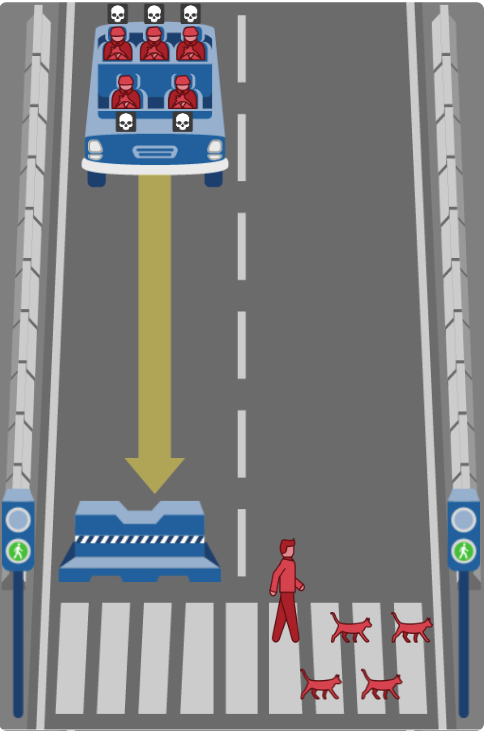
\includegraphics[width=\textwidth]{images/1-left}
            \caption{In this case, the self-driving car with sudden brake failure will continue ahead and crash into a concrete barrier. \textit{This will result in 5 dead homeless people.}\\}
        \end{subfigure}\quad\quad
        \begin{subfigure}{.45\textwidth}
            \centering
            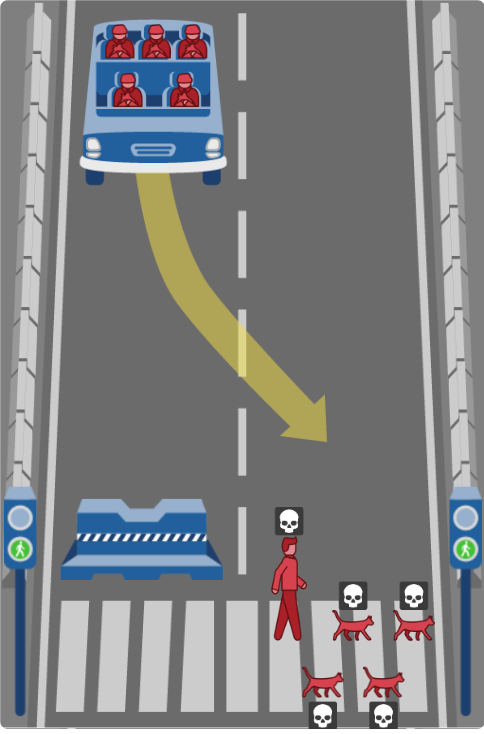
\includegraphics[width=\textwidth]{images/1-right}
            \caption{In this case, the self-driving car with sudden brake failure will swerve and drive through a pedestrian crossing in the other lane. \textit{This will result in 1 dead man, 4 dead cats.}}
        \end{subfigure}

        \caption{First scenario.}
        \label{fig:first}
    \end{figure}

    For the first scenario, described in Figure~\ref{fig:first}, I believe the scenario that should be chosen is the straight into the concrete barrier. This may seem counterintuitive, favoring five human lives over 1 human life and 4 dead animals. However, remember the empathy is with the programmer. The best heuristic is often the simplest one; in this case, the simpler heuristic is going straight into a barricade.

    To further expand, this heuristic \emph{should not} always be used. This heuristic should be used in situations where there are a \emph{comparable} number of passengers and pedestrians.

    \begin{figure}[!h]
        \centering
        \begin{subfigure}{.45\textwidth}
            \centering
            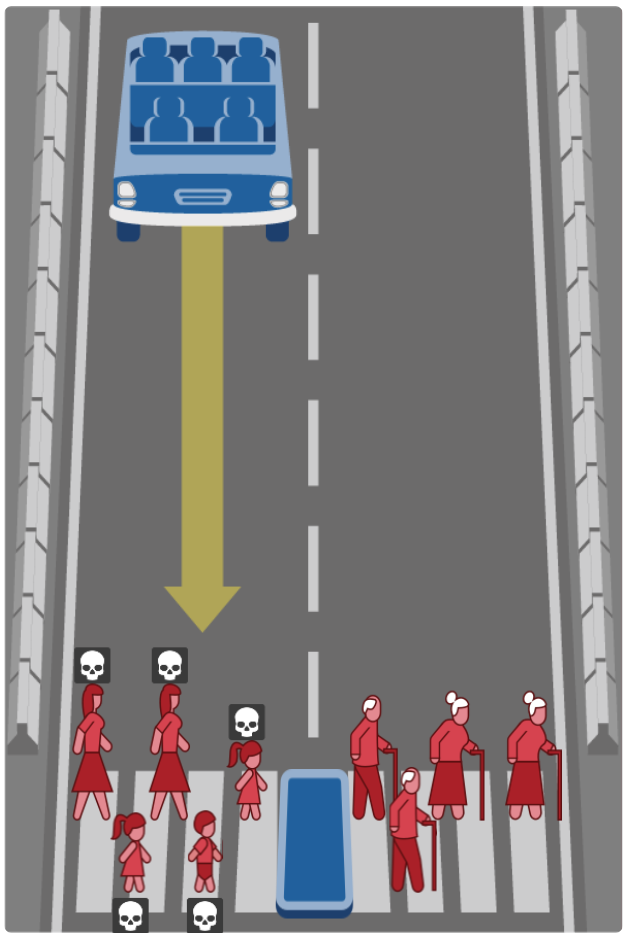
\includegraphics[width=\textwidth]{images/2-left}
            \caption{In this case, the self-driving car with suddent brake failure will continue ahead and drive through a pedestrian crossing ahead. \textit{This will result in 2 women, 2 girls, 1 boy dead.}}
        \end{subfigure}\quad\quad
        \begin{subfigure}{.45\textwidth}
            \centering
            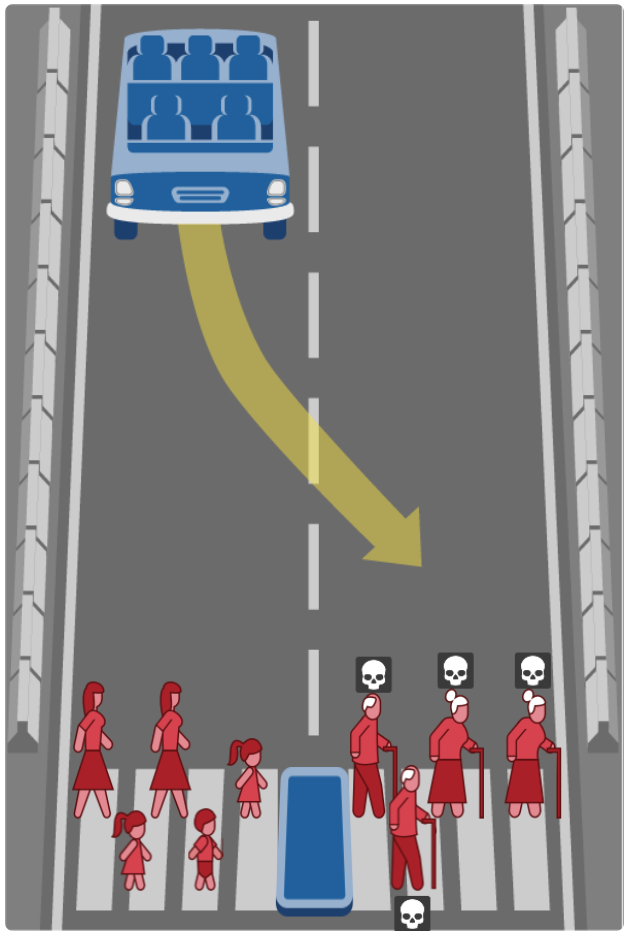
\includegraphics[width=\textwidth]{images/2-right}
            \caption{In this case, the self-driving car with sudden brake failure will swerve and drive through a pedestrian crossing in the other lane.  \textit{This will result in 2 elderly men, 2 elderly women.}}
        \end{subfigure}
        \caption{Second scenarios}
        \label{fig:second}
    \end{figure}

    For the second scenario, described in Figure~\ref{fig:second}, I believe the scenario that should be chosen is to swerve --- contradicting my first decision! This is simply because this is no longer a pedestrian vs.~passenger situation. It is a pedestrian vs.~pedestrian situation. This alternative situation calls for a different heuristic, because it a completely different situation.

    From the perspective of the programmer, both of these situations are a good trade off between simplicity and favorable for the passengers/pedestrians --- and this is something the consumer should want; even though it is not always what the consumer \emph{does} want.
\end{homeworkProblem} \clearpage

\end{document}
